%%%%%%%%%%%%%%%%%%%%%%%%%%%%%%%%%%%%%%
% This poster uses a theme taken from Nathaniel Johnston
% http://www.nathanieljohnston.com/2009/08/latex-poster-template/
%%%%%%%%%%%%%%%%%%%%%%%%%%%%%%%%%%%%%%

\documentclass[final]{beamer}
\usepackage[scale=1.12]{beamerposter}
\usepackage{graphicx}
\usepackage{pstricks}
\usepackage{tikz}
\usepackage[french]{babel}
\usepackage{microtype}
\usepackage{default}
\usepackage{listings}
\usepackage[backend=biber]{biblatex}
\addbibresource{document.bib}
\renewcommand*{\bibfont}{\footnotesize}


%-----------------------------------------------------------
% Define the column width and poster size
% To set effective sepwid, onecolwid and twocolwid values, first choose how many columns you want and how much separation you want between columns
% The separation I chose is 0.024 and I want 4 columns
% Then set onecolwid to be (1-(4+1)*0.024)/4 = 0.22
% Set twocolwid to be 2*onecolwid + sepwid = 0.464
%-----------------------------------------------------------

\newlength{\sepwid}
\newlength{\onecolwid}
\newlength{\twocolwid}
\setlength{\paperwidth}{48in}
\setlength{\paperheight}{36in}
\setlength{\sepwid}{0.024\paperwidth}
\setlength{\onecolwid}{0.22\paperwidth}
\setlength{\twocolwid}{0.464\paperwidth}
\setlength{\topmargin}{-0.5in}
\usetheme{confposter}
\usepackage{exscale}

%-----------------------------------------------------------
% The next part fixes a problem with figure numbering. Thanks Nishan!
% When including a figure in your poster, be sure that the commands are typed in the following order:
% \begin{figure}
% \includegraphics[...]{...}
% \caption{...}
% \end{figure}
% That is, put the \caption after the \includegraphics
%-----------------------------------------------------------

\usecaptiontemplate{
\small
\structure{\insertcaptionname~\insertcaptionnumber:}
\insertcaption}

%-----------------------------------------------------------
% Define colours (see beamerthemeconfposter.sty to change these colour definitions)
%-----------------------------------------------------------

\setbeamercolor{block title}{fg=DarkGray,bg=white}
\setbeamercolor{block body}{fg=DarkGray,bg=white}
\setbeamercolor{block alerted title}{fg=DarkGray,bg=LightGray}
\setbeamercolor{block alerted body}{fg=DarkGray,bg=LightGray}
%-----------------------------------------------------------
% Name and authors of poster/paper/research
%-----------------------------------------------------------

\title{Exécution répartie de partitions interactives}
\author{Jean-Michaël Celerier}
\institute{Laboratoire Bordelais de Recherche en Informatique, Blue Yeti}

\begin{document}
\begin{frame}[fragile,t]    
   \setbeamerfont*{block title}{size=\Large,series=\bfseries}
\begin{columns}[t]
   \begin{column}{\sepwid}\end{column}
     \begin{column}{\onecolwid}
      \begin{block}{Problématique}
          \begin{columns}[t]
              \begin{column}{\onecolwid}\justify
                  Conception d'un logiciel d'écriture temporelle amené à être utilisé en production par des artistes tout en servant de plate-forme de recherche extensible pour des technologies multimédia.
                \end{column}
            \end{columns}        
      \end{block}
     \end{column}
     \begin{column}{\sepwid}\end{column}
     \begin{column}{\twocolwid}
         \begin{block}{Méthode}             
             \begin{columns}[t]	                 
                 \begin{column}{\onecolwid}\justify
                     Conception en entité-composant-système avec hiérarchies symétriques d'entités et de composants. 
                     Plusieurs moteurs opèrent en parallèle, avec une conception modulaire pour étendre le modèle.
                     \end{column}
                     \begin{column}{\onecolwid}\justify
                         Création d'entités sémantiques fortes par héritage, puis d'extensions faibles par composition.
                         Hiérarchie : création automatique de composants enfants à la création de nouvelles entités. 
                        \end{column}
                \end{columns}                 
            \end{block}
      \end{column}
      \begin{column}{\sepwid}\end{column}
      \begin{column}{\onecolwid}
          \begin{block}{Résultats}
          	\begin{columns}[t]
          		\begin{column}{\onecolwid}\justify
                      Plusieurs moteurs sont implémentés de cette manière : il est en pratique souvent nécessaire d'avoir des graphes miroirs du graphe principal avec des données supplémentaires.
          		\end{column}
          	\end{columns}        
            \end{block}
        \end{column}         
   \begin{column}{\sepwid}\end{column}		
\end{columns}

\setbeamerfont*{block title}{size=\Large} 
  \vspace{0.5in}  
  \begin{columns}[t]
    
 \begin{column}{\sepwid}\end{column}
 
 \begin{column}{\onecolwid}
  \begin{beamercolorbox}[wd=\textwidth,colsep=0.05cm]{cboxb}\end{beamercolorbox}
 \end{column}
  
 \begin{column}{\sepwid}\end{column}
  
 \begin{column}{\twocolwid}
  \begin{beamercolorbox}[wd=\textwidth,colsep=0.05cm]{cboxb}\end{beamercolorbox}            
 \end{column}
  
 \begin{column}{\sepwid}\end{column}
 
 \begin{column}{\onecolwid}
  \begin{beamercolorbox}[wd=\textwidth,colsep=0.05cm]{cboxb}\end{beamercolorbox}
 \end{column}         
  
 \begin{column}{\sepwid}\end{column}
\end{columns}
  \vspace{-1ex}  
  \begin{columns}[t]
    \begin{column}{\sepwid}\end{column}
    \begin{column}{\onecolwid}
      \vskip2ex
       \begin{block}{Partitions interactives}
\begin{figure}
    \begin{tikzpicture}[scale=4, every node/.style={scale=0.8}]
\fill (0, 21.6585) circle (0.075) ; % State.1 
\fill (0.801509, 21.6585) circle (0.075) ; % State.2 
\fill (0.801509, 20.5122) circle (0.075) ; % State.3 
\fill (4.1715, 20.5122) circle (0.075) ; % State.4 
\fill (0.801509, 21.387) circle (0.075) ; % State.5 
\fill (3.23104, 21.387) circle (0.075) ; % State.6 
\fill (3.23104, 21.0099) circle (0.075) ; % State.7 
\fill (5, 21.0099) circle (0.075) ; % State.8 
\fill (4.1715, 20.2558) circle (0.075) ; % State.9 
\fill (5, 20.2558) circle (0.075) ; % State.10 
\fill (0.801509, 19.1095) circle (0.075) ; % State.11 
\fill (2.96233, 19.1095) circle (0.075) ; % State.12 
\draw[line width=3pt] (0, 21.6585)  -- (0, 21.6585) ; % TimeNode.0 
\draw[line width=3pt] (0.801509, 21.6585)  -- (0.801509, 19.1095) ; % mule87fens83 
\draw[line width=3pt] (4.1715, 20.5122)  -- (4.1715, 20.2558) ; % zero63aunt55 
\draw[line width=3pt] (3.23104, 21.387)  -- (3.23104, 21.0099) ; % dell37didn59 
\draw[line width=3pt] (5, 21.0099)  -- (5, 20.2558) ; % brow57jill79 
\draw[line width=3pt] (2.96233, 19.1095)  -- (2.96233, 19.1095) ; % many97grid9 
\draw[dashed,line width=3pt] (0, 21.6585)  -- (0.801509, 21.6585) ; % slog45felt83 
\draw[line width=3pt] (0.801509, 20.5122)  -- (4.1715, 20.5122) ; % volume 
\draw[line width=3pt] (0.801509, 20.4122)  -- (4.1715, 20.4122)  -- (4.1715, 19.4122)  -- (0.801509, 19.4122)  -- (0.801509, 20.4122) ;
\draw[line width=3pt] (0.801509, 19.4122)  -- (4.1715, 20.4122) ;
\draw[line width=3pt] (0.801509, 21.387)  -- (3.23104, 21.387) ; % ears55auto57 
\draw[dashed,line width=3pt] (3.23104, 21.0099)  -- (5, 21.0099) ; % cole68beet23 
\draw[line width=3pt] (4.1715, 20.2558)  -- (4.574, 20.2558) ; % nate5just59 
\draw[dashed,line width=3pt] (4.474, 20.2558)  -- (5.71206, 20.2558) ; % nate5just59 
\draw[line width=3pt] (4.714, 20.4088) arc(90:270:0.15) ; % nate5just59 
\draw[line width=3pt] (5.56206, 20.1058) arc(-90:90:0.15) ; % nate5just59 
\draw[line width=3pt] (0.801509, 19.1095)  -- (2.96233, 19.1095) ; % lumiere 
\draw[line width=3pt] (0.801509, 19.0095)  -- (2.96233, 19.0095)  -- (2.96233, 18.0095)  -- (0.801509, 18.0095)  -- (0.801509, 19.0095) ;
\draw[line width=3pt] (0.801509, 18.0095)  -- (2.96233, 19.0095) ;
\draw[line width=3pt] (0.601509, 20.5122)  -- (0.601509, 19.1095) ; % adds31aloe19 
\draw[line width=3pt] (0.601509, 20.5122) arc(180:75:0.2) ; % adds31aloe19 
\draw[line width=3pt] (0.601509, 19.1095) arc(180:285:0.2) ; % adds31aloe19 


\draw (2.1, 21.5199) node {Durée fixe};
\draw (4.104, 21.1099) node {Durée souple};
\draw (2.201509, 20.7) node {Branches conditionnées};
\draw (1.301509, 20) node {Contenu};
\draw (1.301509, 18.6295) node {Contenu};
\draw (5, 21.4099) node {Interaction};
\end{tikzpicture}
\caption{Syntaxe d'une partition interactive}
\end{figure}
Possibilités d'écritures forment un langage de programmation structuré axé sur l'organisation temporelle. 
\textbf{Boucles} et \textbf{hiérarchie}, calcul instantané ou temporel possible via \textbf{Javascript}.
Applications : musique interactive, scénographie et spectacle vivant, contrôle de robots.

Répartition bas-niveau fait déjà partie du formalisme : envoi de messages entre applications, synchronisation, etc.
\end{block}
\begin{block}{Applications visées}
    \begin{itemize}
        \item \textbf{Murs d'écrans} vidéo.
        \item Installations artistiques polyphoniques et ouvertes~: 
        par exemple permettre d'utiliser la présence de \textbf{plusieurs appareils mobiles} 
        lors de l'écriture.
        \item \textbf{Back-up} à chaud des régies de spectacle.
        \item Réduction de gigue sur périphériques embarqué.
    \end{itemize}
\end{block}
      \vskip2ex
      \begin{block}{Existant}
\textbf{Modélisation algorithmique} : réseaux de Petri pour les synchronisations. 
\textbf{Horloges} : Horloges physiques (NTP, PTP), logiques (Lamport clock, vector, matrix) et hybrides.
Approches par intervalles plutôt que par dates : Google TrueTime.
Horloes adaptées à la gestion du temps musical : Ableton Link, Global Metronome.
\textbf{Applications musicales réparties} : Ohm Studio, Splice, Supercollider.
\end{block}
    \end{column}

    \begin{column}{\sepwid}\end{column}
    \begin{column}{\twocolwid}
      \begin{columns}[t,totalwidth=\twocolwid]
        \begin{column}{\onecolwid}\vspace{-.67in}
            \vskip2ex
            \begin{block}{Synchronisation des macro-structures}
	Programme temporel : \textbf{scénario}. 
	
	Trois modes d'exécution : 
	\begin{itemize}
		\item Indépendant
		\item Partagé
		\item Mixte
	\end{itemize}
\end{block}
        \end{column}
        \begin{column}{\onecolwid}\vspace{-.67in}
            \vskip2ex
            \begin{block}{Synchronisation des micro-structures}
    Dans le cas d'une exécution partagée d'un scénario, il convient de définir la sémantique d'exécution des points de synchronisation, des conditions, et des vitesses de contraintes, en mode réparti. 
   
    C'est fait via deux caractéristiques:~\\
    La \textbf{synchronisation}~:
	\begin{itemize}
		\item \textbf{Mode synchrone}~: on respecte la sémantique d'exécution des partitions interactives au prix d'une latence de synchronisation.
		\item \textbf{Mode asynchrone}~: on ne respecte pas la sémantique avant-après. La fin de l'exécution d'un objet peut survenir quelques millisecondes après le début de l'exécution de l'objet suivant.
	\end{itemize}

Le \textbf{délai de propagation}~:
\begin{itemize}
    \item \textbf{Propagation instantanée}~: dès qu'une information est disponible dans le système, les clients qui en dépendent en sont informés et peuvent y réagir immédiatement. 
    \item \textbf{Propagation compensée}~: quand une information est disponible dans le système, on estime la date minimale à partir de laquelle tous les clients peuvent être informés en fonction de la latence entre machines. 
    Elles reçoivent toutes un ordre qu'elles sont sensées exécuter à cette date. 
    C'est utile si on désire par exemple une bonne synchronisation entre vidéos.
\end{itemize}

Via des annotations, le compositeur peut définir le type de répartition qu'il souhaite sur chaque objet.

\begin{figure}
	\begin{tikzpicture}[scale=4]
	\fill (0, 9.98122) circle (0.075) ; % State.0 
\fill (2.44792, 9.98122) circle (0.075) ; % State.1 
\fill (2.44792, 9.41005) circle (0.075) ; % State.2 
\fill (5, 9.41005) circle (0.075) ; % State.3 
\draw[line width=1pt] (0, 9.98122)  -- (0, 9.98122) ; % TimeNode.0 
\draw[line width=1pt] (2.44792, 9.98122)  -- (2.44792, 9.41005) ; % numb47vine94 
\draw[line width=1pt] (5, 9.41005)  -- (5, 9.41005) ; % faze44greg1 
\draw[line width=1pt] (0, 9.98122)  -- (2.44792, 9.98122) ; % dido10rend91 
\draw (1.22396, 10.1812) node {$C_1: G_1$}; % dido10rend91 
\draw[line width=1pt] (2.44792, 9.41005)  -- (5, 9.41005) ; % taut8hews94 
\draw (3.72396, 9.61005) node {$C_2: G_2$}; % taut8hews94 

	\end{tikzpicture}
	\begin{tikzpicture}[scale=4]
	\fill (0, 12.3782) circle (0.075) ; % State.0 
\fill (2.25275, 12.3782) circle (0.075) ; % State.1 
\fill (0, 11.5717) circle (0.075) ; % State.2 
\fill (2.33516, 11.5717) circle (0.075) ; % State.3 
\fill (5, 11.5717) circle (0.075) ; % State.4 
\draw[line width=3pt] (0, 12.3782)  -- (0, 11.5717) ; % TimeNode.0 
\draw[line width=3pt] (2.25275, 12.3782)  -- (2.25275, 12.3782) ; % said66toil5 
\draw (2.25275, 12.6282) node {$M_1$}; % said66toil5 
\draw[line width=3pt] (2.33516, 11.5717)  -- (2.33516, 11.5717) ; % dear17tick57 
\draw (2.33516, 11.8217) node {$T_1$}; % dear17tick57 
\draw[line width=3pt] (5, 11.5717)  -- (5, 11.5717) ; % pane76toll8 
\draw[line width=3pt] (0, 12.3782)  -- (2.25275, 12.3782) ; % mask27tara32 
\draw (1.12637, 12.5782) node {$C_1$}; % mask27tara32 
\draw[dashed,line width=3pt] (0, 11.5717)  -- (2.33516, 11.5717) ; % acid4ball90 
\draw (1.16758, 11.7717) node {$C_{1\rightarrow2}$}; % acid4ball90 
\draw[line width=3pt] (2.33516, 11.5717)  -- (5, 11.5717) ; % ride82vine29 
\draw (3.66758, 11.7717) node {$C_2$}; % ride82vine29 

	\end{tikzpicture}
	\begin{tikzpicture}[scale=4]
	\fill (0, 12.3782) circle (0.075) ; % State.0 
\fill (2.25275, 12.3782) circle (0.075) ; % State.1 
\fill (0, 11.5717) circle (0.075) ; % State.2 
\fill (2.33516, 11.5717) circle (0.075) ; % State.3 
\fill (5, 11.5717) circle (0.075) ; % State.4 
\draw (0.25, 12.6282) node {$M_1$};
\draw[line width=1pt] (0, 12.3782)  -- (0, 11.5717) ; % TimeNode.0 
\draw (0.25, 11.8217) node {$T_1$};
\draw[line width=1pt] (2.25275, 12.3782)  -- (2.25275, 12.3782) ; % said66toil5 
\draw[line width=1pt] (2.33516, 11.5717)  -- (2.33516, 11.5717) ; % dear17tick57 
\draw (2.33516, 11.8217) node {}; % dear17tick57 
\draw[line width=1pt] (5, 11.5717)  -- (5, 11.5717) ; % pane76toll8 
\draw[line width=1pt] (0, 12.3782)  -- (2.25275, 12.3782) ; % mask27tara32 
\draw (1.12637, 12.5782) node {$C_1$}; % mask27tara32 
\draw[line width=1pt] (0, 11.5717)  -- (2.33516, 11.5717) ; % acid4ball90 
\draw (1.16758, 11.7717) node {$C_{1\rightarrow2}$}; % acid4ball90 
\draw[line width=1pt] (2.33516, 11.5717)  -- (5, 11.5717) ; % ride82vine29 
\draw (3.66758, 11.7717) node {$C_2$}; % ride82vine29 

	\end{tikzpicture}
	\caption{De haut en bas : la partition que le compositeur exprime, sa version lorsque répartie en mode asynchrone pré-calculé et sa version lorsque répartie en mode synchrone compensé.}
\end{figure}
\end{block}
        \end{column}
      \end{columns}
      \vskip2.5ex
      \begin{block}{}
          \begin{figure}
              \centering
              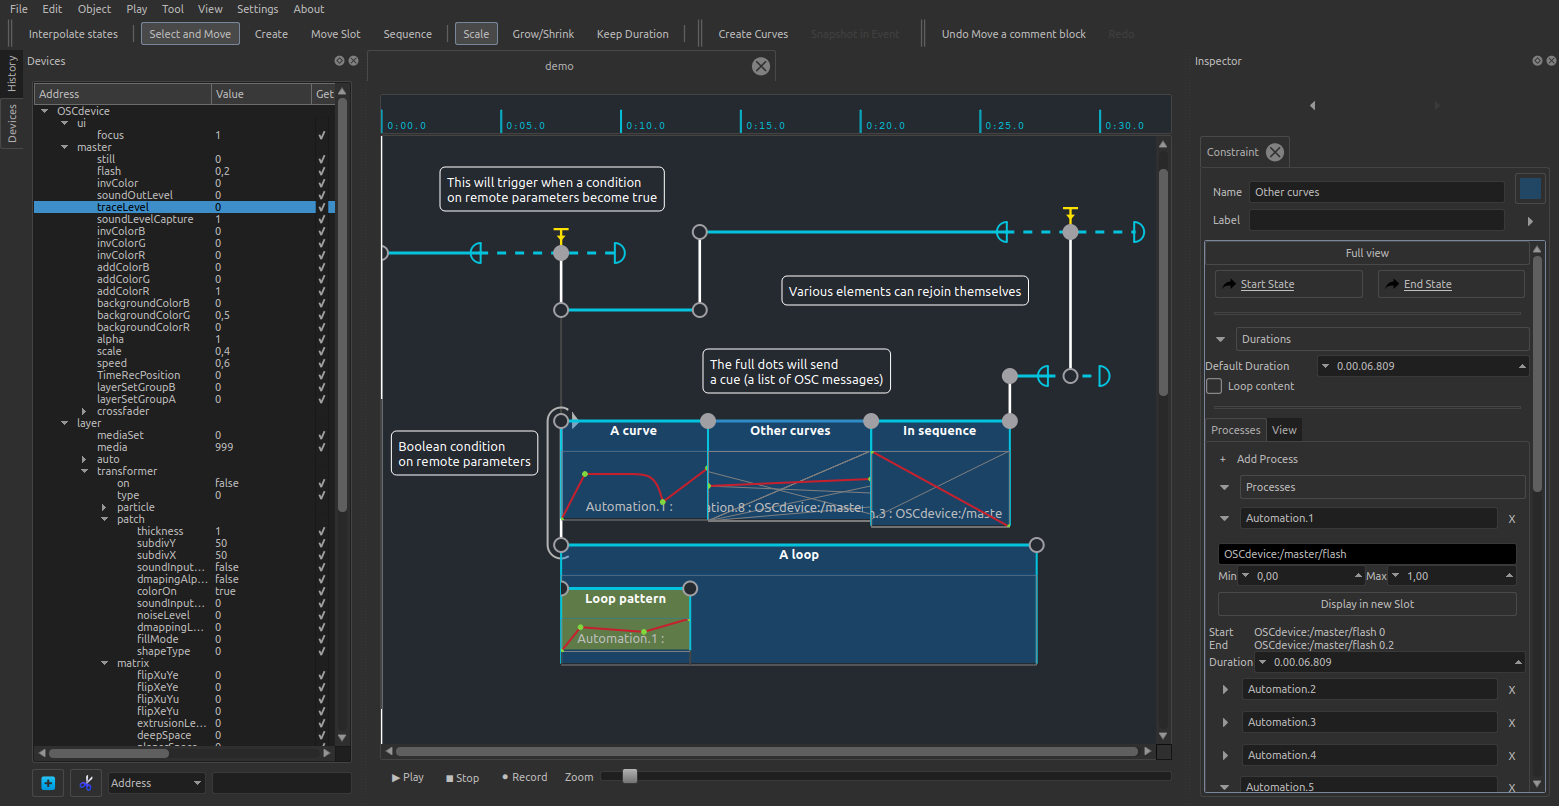
\includegraphics[width=\textwidth]{images/iscore.png}
              \caption{Un scénario d'exemple i-score}
            \end{figure}
      \end{block}
  \end{column}
  \begin{column}{\sepwid}\end{column}
  \begin{column}{\onecolwid}
    \vskip2ex
    \begin{block}{Prochains objectifs}
	\begin{itemize}
		\item Évolution vers édition répartie de partitions interactives, pendant leur exécution. Objectif~: permettre à plusieurs régisseurs (son, lumière) de garder la main sur une même exécution.
		\item Comportements de groupe~: utiliser les informations provenant de chaque client, pour générer de nouveaux contenus. Par exemple, étant donné plusieurs téléphones portables, pouvoir utiliser les capteurs intégrés et travailler avec le comportement moyen sur ce groupe.
	\end{itemize}
\end{block}
    \vskip2ex
    \begin{block}{Informations complémentaires}
    	% Site web
    	% Article
      {Articles sur ce sujet~:
      \begin{itemize}
        \item Modèles formels sur lesquels se base i-score~:~\\\cite{allombert_system_2007,arias_modelling_2014}.
        \item Paradigme graphique OSSIA~:~\cite{celerier_ossia:_2015}.
      \end{itemize}
      \vspace{0.1in}\noindent i-score peut être téléchargé librement sur
      \begin{itemize}
        \item \url{www.i-score.org}
      \end{itemize}}
\end{block}
    \vskip2ex
    \begin{block}{Références}
        \footnotesize\printbibliography
    \end{block}
    \vskip2ex
  \end{column}
  \begin{column}{\sepwid}\end{column}			% empty spacer column
 \end{columns}
\end{frame}
\end{document}

